\documentclass[MachineLearning]{subfiles}
\begin{document}

%@@@@@@@@@@@@@@@@@@@@@@@@@@@@@@
% summarizes lecture 3
% author: Benjamin Ellenberger

\section{Regression}
In statistics, regression analysis is a statistical process for estimating the relationships among variables (one independent variable Y and one or more independent variable (\(X_1,\ldots,X_d\))). More specifically, regression analysis helps one understand how the typical value of the dependent variable (or 'criterion variable') changes when any one of the independent variables is varied, while the other independent variables are held fixed. A
model of the relationship is hypothesized, and estimates of the parameter values are used to develop an estimated regression equation. Various
tests are then employed to determine if the model is satisfactory.If the model is
deemed satisfactory, the estimated re- gression equation can be used to predict the value of the dependent variable given values for the independent variables. (Source: Wikipedia and Encyclopedia Britannica on Regression)\\
\begin{itemize}
\item Object space \(\mathcal{O}\)
\item Measurement/Feature space \(\mathcal{F} = \R^d \times \R\)
\item Data \(\mathcal{Z} = \{(x_i,y_i) \in \R^d \times \R : 1 \geq i \geq n\}\)
\end{itemize}
\textbf{The problem of regression}: What is the optimal estimate of a function \(f: \R^d \rightarrow \R\) based on noisy data \(y_i = f(x_i) + \epsilon_i\)?\\
\textbf{Solution:} The regression function: \(y(x) = \mathbb{E}\{y | X=x\} = \int_{\Omega} y p(y|X=x)dy\)\\
How many data are required to estimate a model or a regression function given a
hypothesis class (set of possible regression functions)?
\subsection{Linear Regression}
Linear regression comes in a closed form solution.
\begin{figure}[H]
\centering
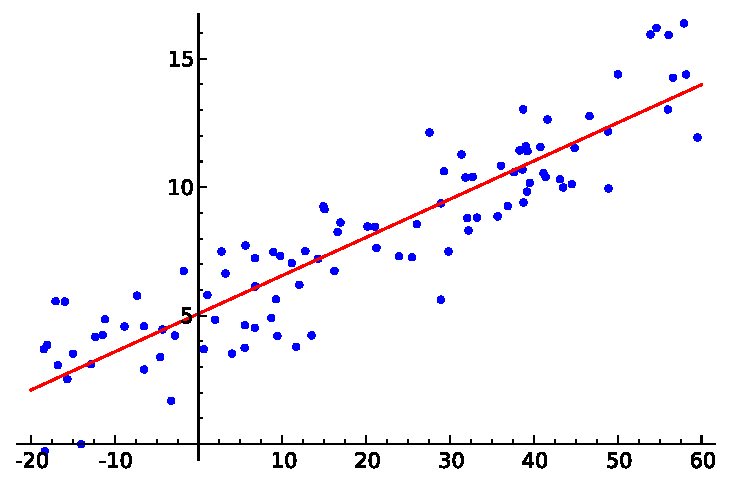
\includegraphics[width=0.5\linewidth]{figs/Linear_regression}
\caption{Linear regression of data}
\end{figure}
Given a vector of inputs \(X^T=(X_1,\ldots,X_d)\). The output variable (also called response variable) is predicted via the model\\
\[Y = \beta_0 + \sum^d_{j=1} X_j\beta_j,~~ Y \in \R\]
\(\beta_0\) is called bias(Machine Learning) or intercept (Statistics). We extend the X vector with an \(X_0 = 1\) and we can include the bias \(\beta_0\) into the vector of \(\beta\)s and can write Y in matrix form: \(Y = X^T\beta,~~X,\beta \in \R^{d+1}\)
\subsubsection{Training of the Linear Regressor: Residual Sum of Squares(RSS)}
Training of an accurate Predictor = Minimize the residual sum of squares between the actual value \(y\) and the predicted \(\overline{X}\beta\):\\
\[RSS(\beta) = \sum^{n}_{i=1}(y_i-x_i^T\beta)^2\] or matrix notation \[RSS(\beta) = (y-\overline{X}\beta)^T(y-\overline{X}\beta),~~X\in \R^n \times \R^{d+1}\] \(\text{(Each row of } \overline{X} \text{ is an input vector } X, y \text{ is an n-vector of the outputs in the training set})\)\\\\
We find the minimum RSS by differentiating w.r.t. \(\beta\)\\ 
\begin{align}
&\rightarrow X^T(y-X\beta) = 0\\
&\rightarrow\hat{\beta} = (X^TX))^{-1}X^Ty~~(\text{Solution for nonsingular} X^TX)
\end{align}
\subsubsection{Prediction via the Trained Linear Regressor}
\[\hat{y} = X \hat{\beta} = X(X^T X)^{-1} X^T y\]
The matrix \(X(X^T X)^{-1} X^T\) is sometimes called the hat matrix
which is an orthogonal projection on the space spanned by the columns of X.
\subsubsection{Perturbation of Linear Regressor with Gaussian Noise}
Gaussian noise \(\epsilon\) with \(\mathcal{E}(\epsilon) = 0, \mathcal{V} = \sigma^2\)
\begin{proof}
\begin{align}
Y &= \mathbb{E}(Y|X_1 , \ldots , X_d) + \epsilon\\
&= \beta_0 + \sum^d_{j=1} X_j \beta_j + \epsilon\\
&= X\beta + \epsilon
\end{align}
Meaning that gaussian noise does not perturb the estimator.
\end{proof}

\subsubsection{Optimality of Least Squares Estimate}
The least squares estimate of the parameter \(\beta\) has the smallest variance among all linear unbiased estimates.\\
We want to predict a. Prediction \(\hat{\theta}\) is a linear function \(c_0^Ty = \overbrace{a^T (X^T X)^{-1} X^T}^{c_0} y\) of the response vector y.
\begin{proof}

\(a^T \hat{\beta}\) is unbiased since the expectation \(\mathbb{E}\) yields
\begin{align}
\mathbb{E}(a^T \hat{\beta}) &= \mathbb{E}(a^T (X^T X)^{-1} X^T y)\\
&= a^T (X^T X)^{-1} X^T \mathbb{E}(X\beta + \epsilon)\\
&= a^T (X^T X)^{-1} X^T (X\beta + \underbrace{\mathbb{E}(\epsilon)}_{=0} ) = a^T \beta\\
\end{align}
Variance of \(a^T\hat{\beta}\)
\begin{align}
\mathbb{V}(a^T \hat{\beta}) &= \mathbb{V}\Big( a^T \underbrace{(X^T X)^{-1} X^T \overbrace{(X\beta + \epsilon)}^{y}}_{\hat{\beta}}\Big)\\
&= \underbrace{\mathbb{V}(a^T \beta)}_{=0} +\mathbb{V}\left(a^T (X^T X)^{-1} X^T \epsilon\epsilon^T X(X^T X)^{-1} a\right)
= \sigma^2 a (X^T X)^{-1} a
\end{align}
The cross-correlations are linear in \(\epsilon\) and, therefore, they vanish.\\\\
Alternative unbiased linear estimator (to show the least squares estimator is the best)
\begin{align}
\hat{\theta} &= c^T y = a^T \hat{\beta} + a^T Dy\\
\mathbb{E}(c^T y) &= \mathbb{E}(a^T \hat{\beta}) + \mathbb{E}(a^T Dy) = a^T \beta + \mathbb{E} a^T D(X\beta + \epsilon)\\
&= a^T \beta + a^T DX\beta + a^T D \underbrace{\mathbb{E}(\epsilon)}_{=0} = a^T \beta\\
\end{align}
The (unbiasedness) condition \(\mathbb{E}(c^T y) = a^T \beta\) implies \(DX = 0\).
\end{proof}
Gauss-Markov Theorem proves \(\mathbb{V}(a^T\hat{\beta}) \leq \mathbb{V}(c^Ty)\)
\subsection{Ridge Regression}
\subsection{LASSO}
\subsection{Nonlinear Regression by basis expansion}
\subsection{Wavelet regression}
\subsection{Bias variance Tradeoff}
\subsection{Gaussian Processes}
\end{document}